\chapter{System Architecture}

\section{Overview}
The Face Recognition Attendance System is a sophisticated application that combines computer vision, parallel processing, and database management to provide efficient attendance tracking through facial recognition.

\section{Core Technologies}
\begin{itemize}
    \item \textbf{Programming Language:} Python 3.7+
    \item \textbf{GUI Framework:} Tkinter
    \item \textbf{Computer Vision:} OpenCV, InsightFace
    \item \textbf{Database:} SQLite with SQLAlchemy ORM
\end{itemize}

\section{System Components}
\begin{figure}[H]
\centering
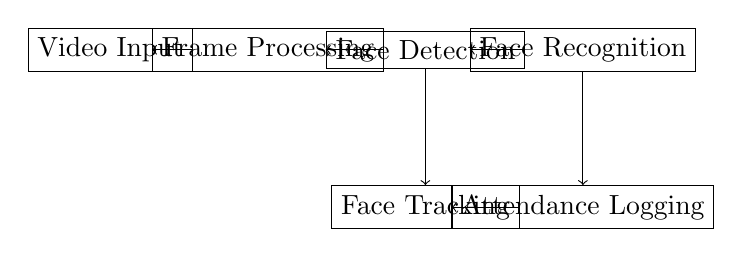
\begin{tikzpicture}[node distance=2cm]
    \node (video) [draw, rectangle] {Video Input};
    \node (process) [draw, rectangle, right of=video] {Frame Processing};
    \node (detect) [draw, rectangle, right of=process] {Face Detection};
    \node (recog) [draw, rectangle, right of=detect] {Face Recognition};
    \node (track) [draw, rectangle, below of=detect] {Face Tracking};
    \node (log) [draw, rectangle, below of=recog] {Attendance Logging};
    
    \draw[->] (video) -- (process);
    \draw[->] (process) -- (detect);
    \draw[->] (detect) -- (recog);
    \draw[->] (detect) -- (track);
    \draw[->] (recog) -- (log);
    \draw[->] (track) -- (log);
\end{tikzpicture}
\caption{System Architecture Overview}
\end{figure}

\section{Core Features}
\begin{enumerate}
    \item \textbf{Real-time Face Detection}
    \begin{itemize}
        \item Multi-scale detection
        \item High-performance processing
        \item Configurable detection parameters
    \end{itemize}
    
    \item \textbf{Face Recognition}
    \begin{itemize}
        \item Deep learning-based recognition
        \item Face embedding generation
        \item Confidence scoring
    \end{itemize}
    
    \item \textbf{Attendance Management}
    \begin{itemize}
        \item Automatic check-in/check-out
        \item Real-time logging
        \item Report generation
    \end{itemize}
    
    \item \textbf{User Interface}
    \begin{itemize}
        \item Live video feed display
        \item Control panel
        \item Status notifications
    \end{itemize}
\end{enumerate}

\section{System Requirements}

\subsection{Hardware Requirements}
\begin{itemize}
    \item CPU: Multi-core processor
    \item RAM: Minimum 8GB
    \item Storage: 1GB+ for database and face samples
    \item Camera: HD webcam capability
\end{itemize}

\subsection{Software Dependencies}
\begin{lstlisting}[language=Python]
# Core Requirements
opencv-python>=4.5.0
numpy>=1.19.0
insightface>=0.6.0
sqlalchemy>=1.4.0
pillow>=8.0.0
scipy>=1.7.0

# Optional Dependencies
pandas  # for attendance analysis
matplotlib  # for visualization
onnxruntime  # for optimized inference
\end{lstlisting}

\section{Directory Structure}
\begin{lstlisting}
project_root/
├── src/
│   ├── database/
│   ├── utils/
│   └── face_recognition/
├── ui/
│   ├── components/
│   └── theme/
├── tests/
├── face_data/
│   ├── models/
│   └── database/
└── documentation/
\end{lstlisting}

\section{Configuration Management}
\begin{lstlisting}[language=Python]
# config.py
class Config:
    # Video capture settings
    CAMERA_RESOLUTION = (1920, 1080)
    FPS_TARGET = 30
    FRAME_BUFFER_SIZE = 30
    
    # Face detection settings
    DETECTION_INTERVAL = 2
    CONFIDENCE_THRESHOLD = 0.6
    
    # Database settings
    DATABASE_URL = "sqlite:///database.sqlite"
    POOL_SIZE = 5
    MAX_OVERFLOW = 10
\end{lstlisting}